%\title{LaTeX Portrait Poster Template}
%%%%%%%%%%%%%%%%%%%%%%%%%%%%%%%%%%%%%%%%%
% a0poster Portrait Poster
% LaTeX Template
% Version 1.0 (22/06/13)
%
% The a0poster class was created by:
% Gerlinde Kettl and Matthias Weiser (tex@kettl.de)
% 
% Adapter by Jens Buysse for Hogeschool Gent
% This template has been downloaded from:
% http://www.LaTeXTemplates.com
%
% License:
% CC BY-NC-SA 3.0 (http://creativecommons.org/licenses/by-nc-sa/3.0/)
%
%%%%%%%%%%%%%%%%%%%%%%%%%%%%%%%%%%%%%%%%%

%----------------------------------------------------------------------------------------
%	PACKAGES AND OTHER DOCUMENT CONFIGURATIONS
%----------------------------------------------------------------------------------------

\documentclass[a0,portrait]{a0poster}

\usepackage{multicol} % This is so we can have multiple columns of text side-by-side
\columnsep=100pt % This is the amount of white space between the columns in the poster
\columnseprule=3pt % This is the thickness of the black line between the columns in the poster

\usepackage[svgnames]{xcolor} % Specify colors by their 'svgnames', for a full list of all colors available see here: http://www.latextemplates.com/svgnames-colors

\usepackage{times} % Use the times font
%\usepackage{palatino} % Uncomment to use the Palatino font

\usepackage{graphicx} % Required for including images
\graphicspath{{figures/}} % Location of the graphics files
\usepackage{booktabs} % Top and bottom rules for table
\usepackage[font=small,labelfont=bf]{caption} % Required for specifying captions to tables and figures
\usepackage{amsfonts, amsmath, amsthm, amssymb} % For math fonts, symbols and environments
\usepackage{wrapfig} % Allows wrapping text around tables and figures
\usepackage[export]{adjustbox}

\begin{document}

%----------------------------------------------------------------------------------------
%	POSTER HEADER 
%----------------------------------------------------------------------------------------

% The header is divided into two boxes:
% The first is 75% wide and houses the title, subtitle, names, university/organization and contact information
% The second is 25% wide and houses a logo for your university/organization or a photo of you
% The widths of these boxes can be easily edited to accommodate your content as you see fit

\begin{minipage}[t]{0.75\linewidth}
\VeryHuge \color{HoGentAccent1} \textbf{Natuurlijke Taal omzetten \\naar Programmeertaal door middel van Artifici\"ele Intelligentie} \color{Black}\\ % Title
%\Huge\textit{Ondertitel (eventueel)}\\[2.4cm] % Subtitle
\huge \textbf{Leroy Preben, Serruys Karel, Van Impe Steven}\\[0.5cm] % Author(s)
\huge Hogeschool Gent, Valentin Vaerwyckweg 1, 9000 Gent\\[0.4cm] % University/organization
\Large \texttt{preben.leroy.w1789@student.hogent.be} \\
\end{minipage}
%
\begin{minipage}[t]{0.25\linewidth}

\includegraphics[width=13cm,right]{figures/HG-woordmerk.jpg} 

\end{minipage}

\vspace{1cm} % A bit of extra whitespace between the header and poster content

%----------------------------------------------------------------------------------------

\begin{multicols}{2} % This is how many columns your poster will be broken into, a portrait poster is generally split into 2 columns

%----------------------------------------------------------------------------------------
%	ABSTRACT
%----------------------------------------------------------------------------------------

\color{HoGentAccent1} % Navy color for the abstract

\begin{abstract}
Deze bachelorproef staat in het teken van artifici\"ele intelligentie en de mogelijkheid om door middel van AI en natuurlijke taal programmeercode te laten genereren. Hiervoor werd er in een eerste fase een literatuurstudie uitgevoerd naar de reeds bestaande mechanismen en hun achterliggende technieken, om in een tweede fase een aantal mechanismen uit te testen. Op die manier werd er getracht een antwoord te geven op de vraag of het mogelijk is om code te genereren door middel van AI en op basis van natuurlijke taal.
\end{abstract}
%----------------------------------------------------------------------------------------
%	INTRODUCTION
%----------------------------------------------------------------------------------------

\color{HoGentAccent1} 
\section*{Introductie}
\color{black}
\color{black}
Artificiële intelligentie is reeds een hot topic in onze maatschappij. Tegenwoordig kan het overal in toegepast worden. Zo wordt het gebruikt in een aantal toepassingen zoals gezichtsherkenning, zelfrijdende auto’s, \dots. Maar wordt het ook voor andere toepassingen de standaard?

Gartner voorspeld dat tegen 2022 slimme technologieën en robots, op basis van artifici\"ele intelligentie, taken kunnen overnemen uit de geneeskunde en de IT. In dit onderzoek gaat het niet over het algemene aspect dat artifici\"ele intelligentie alles zou overnemen.

\begin{center}\vspace{1cm}
	
\includegraphics[width=1.0\linewidth]{Gartner-logo1}
	\captionof{figure}{\color{HoGentAccent5} Logo Gartner. Gartner is een onderzoekbureau in de IT-sector.}
\end{center}\vspace{1cm}

Hier gaan we dieper in op het feit dat AI de ICT drastisch kan veranderen. Zeker voor de programmeurs onder de ICT’ers. Daarom wordt in deze Bachelorproef een onderzoek gedaan naar de mogelijkheid om code te laten genereren door middel van AI vanuit natuurlijke taal.

De vragen die je aan het systeem zou stellen, moeten wel een functioneel karakter hebben. De functionele specificaties van het te bouwen programma moeten in de vraag voorkomen. Bij deze specificaties wordt er helder beschreven waaraan het programma moet voldoen. Hoe duidelijker de vraag aan het systeem, hoe gedetailleerder het systeem code zou kunnen schrijven.

In de eerste plaats kunnen deze technieken in de toekomst gebruikt worden door softwareontwikkelingsbedrijven. Daarnaast kunnen bedrijven die databank-transacties regelen ook de vruchten plukken van dit onderzoek.

%----------------------------------------------------------------------------------------
%	GEOLOGY
%----------------------------------------------------------------------------------------

\color{Black} % DarkSlateGray color for the rest of the content
\color{HoGentAccent1} 
\section*{Experimenten}
\color{black}

In eerste instantie werd er een uitgebreide literatuurstudie uitgevoerd. Tijdens de uitvoering van dit onderzoek werden een aantal algoritmen besproken voor de generatie van code. Deze algoritmen kunnen onderverdeeld worden in een aantal categorieën. 

\begin{itemize}
	\item Programma Generatie
		\begin{itemize}
			\item Microsoft DeepCoder
			\item AI Programmer
		\end{itemize}
	\item Machine Learning
	\begin{itemize}
		\item Google AutoML
	\end{itemize}
	\item SQL Generatie
	\begin{itemize}
		\item Seq2SQL
		\item SQLNet
		\item NLIDBS
		\item NL2Prog
	\end{itemize}
\end{itemize}

Als experiment werden er twee van deze algoritmen, namelijk Seq2SQL en SQLNet, uitgetest. Ook werd er hier ook een derde item uitgetest, namelijk WikiSQL. Zowel het Seq2SQL-model als het SQLNet-model maken gebruik van WikiSQL om de algoritmen te trainen.

\begin{center}\vspace{1cm}
	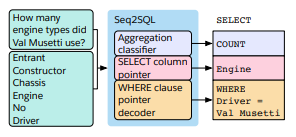
\includegraphics[width=1.0\linewidth]{seq2sqlmodel}
	\captionof{figure}{\color{HoGentAccent5} Het Seq2SQL-model. Een SQL-query bestaat meestal uit 3 onderdelen: een aggregatie-operator (bijvoorbeeld SUM of COUNT), de kolom waarop de query dient uitgevoerd te worden en de WHERE-clause. Seq2SQL zorgt ervoor dat een vraag direct in zo'n vorm kan gegoten worden}
\end{center}\vspace{1cm}

\begin{center}\vspace{1cm}
	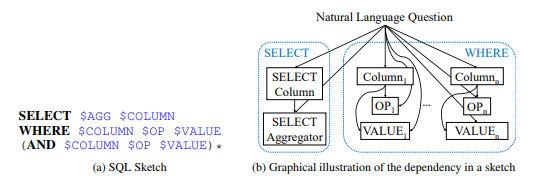
\includegraphics[width=1.0\linewidth]{sqlnetmodel}
	\captionof{figure}{\color{HoGentAccent5} Het SQLNet-model. Figuur a: SQL-sleutelwoorden (SELECT, WHERE en AND) worden in een schets weergegeven. De operatoren die starten met het \$ teken dienen ingevuld te worden. De AND-clause dient niet altijd ingevuld te worden. In figuur b kan de zogenaamde afhankelijkheidsgrafiek teruggevonden worden.}
\end{center}\vspace{1cm}

Elk model werd kort aangehaald. Vervolgens werd er getracht de opbouw van het algoritme (op basis van de gevonden Github-repositories) zo gedetaileerd mogelijk uit te schrijven. Vervolgens werden de algoritmen uitgetest. Alle nodige commando's werden uitgeschreven. Elk commando wordt ook grondig en gedetaileerd uitgelegd.

Indien het mogelijk was de algoritmen uit te voeren, werden de verkregen resultaten vergeleken met de resultaten die vermeld werden in de papers. Indien het niet mogelijk was de algoritmen uit te voeren, werden er oorzaken gezocht en eventuele oplossingen geprobeerd om alles toch werkende te krijgen. 

Eigenlijk was het ook de bedoeling om in een tweede fase van dit experiment de algoritmen uit te testen om een andere dataset. Door enkele problemen met de onderzochte algoritmen is dit helaas niet gelukt.

%------------------------------------------------

\color{HoGentAccent1} 
\section*{Conclusies}
\color{black}
Op basis van het complete onderzoek kan er geconcludeerd worden dat het mogelijk is om door middel van artifici\"ele intelligentie en op basis van natuurlijke taal programmeercode te genereren. Tools en algoritmen die hiervoor kunnen gebruikt worden zijn onder andere Microsoft DeepCoder, NLIDBS en NL2Prog.

Op basis van de uitgevoerde experimenten dient er hierbij wel een kanttekening gemaakt te worden. De uitvoering van zowel het Seq2SQL-algoritme, het SQLNet-algoritme als het WikiSQL-algoritme staat nog niet volledig op punt. Ofwel waren er problemen met de training van het algoritme, ofwel was het gewoon niet mogelijk het algoritme uit te voeren. 

De complete generatie van programmeercode is, in de praktijk, enkel mogelijk voor de generatie van programmeertalen die behoren tot de vierde generatie. Deze programmeertalen leunen dicht aan tegen de natuurlijke taal. Tools zoals Microsoft DeepCoder of Google AutoML genereren niet echt code, maar helpen toch bij het makkelijker maken van het werk van een IT'er.
%----------------------------------------------------------------------------------------
%	FORTHCOMING RESEARCH
%----------------------------------------------------------------------------------------
\color{HoGentAccent1} 
\section*{Toekomstig onderzoek}
\color{black}

Code genereren door middel van AI op basis van natuurlijke taal is een nieuwe techniek. De nodige modellen voor generatie zijn nog niet volledig en zullen in de loop der tijd uitgebreider en beter worden. Net zoals dat artifici\"ele intelligentie ook nog altijd zal blijven verbeteren. In de praktijk blijkt dat nog enkel maar Google’s AutoML compleet operationeel is. Andere mechanismen zijn deels operationeel, maar de meeste hebben nog meer onderzoek nodig.


%----------------------------------------------------------------------------------------

\end{multicols}
\end{document}